\section{\textbf{The Simulation Environment}} \label{sec:Environment}

	The Open Racing Car Simulator (TORCS) is a platform that is a widely used for benchmarking AI, renowned for its highly credible physics modeling engine and yet user-friendly interface for car racing simulation~\cite{TORCS}. One of the	many other qualities of this open-source simulator is its portability, concerning multi-platform environments - such as different operational systems and architectures - and support to the programming languages C and C++.

\subsection{TORCS} \label{subsec:TORCS}
	
	TORCS is a computer simulation that serves both as an ordinary car racing game and as a research platform~\cite{2009}, making it possible for everyone to create a pilot through coding. The interface with this platform occurs by means of a sensor-based interaction system in which the developer is able to interpret received parameters of the car - such as speed in X, Y and even Z axes - and control the car through programming its actuators, some of which are acceleration and steering.
	
	Another credibility factor for this platform is its non-punctual cars, which interact with each other in the races by a life-like collision system. Nevertheless, TORCS is still a simulator, and its limitations, along with the defined racing environment and the modeled car, are more than likely to affect any results obtained. This is an inherited characteristic of any real-life problem simulation, what in academia is denominated \emph{reality gap}~\cite{RG}, and it stems from the simplifications made concerning the car models, the technical features of the tracks, and so forth.

\subsection{The SCR Championship} \label{subsec:SCRC}

	The Simulated Car Racing Championship (SCRC) is an example of a well-known competition which utilizes TORCS as interface~\cite{SCR}. Being an event joining three competitions held at major scientific conferences, such as \emph{IEEE Congress on Evolutionary Computation}~\footnote{http://www.cec2015.org/}, \emph{Genetic and Evolutionary Computation Conference}~\footnote{http://www.sigevo.org/gecco-2015/} and \emph{IEEE Conference on Computational Intelligence and Games}~\footnote{http://www.ieee-cig.org/}, it is an accepted metric of evaluation in the fields of Evolutionary Computation and Computational Intelligence regarding Games.
	
	In the SCRC, some of the information about the racing execution remains hidden from the controllers, such as the geometrical format of the track and its category. The communication between this championship and TORCS is made through a client-server interface, with each player receiving information from the server regarding the sensors of the car, and in return providing actuator values that determine how the controller is supposed to drive the car. Figure~\ref{Fig:1} illustrates the data available at the TORCS and client - controller - layer of abstraction.

   	\begin{figure}[h]
		\centering
		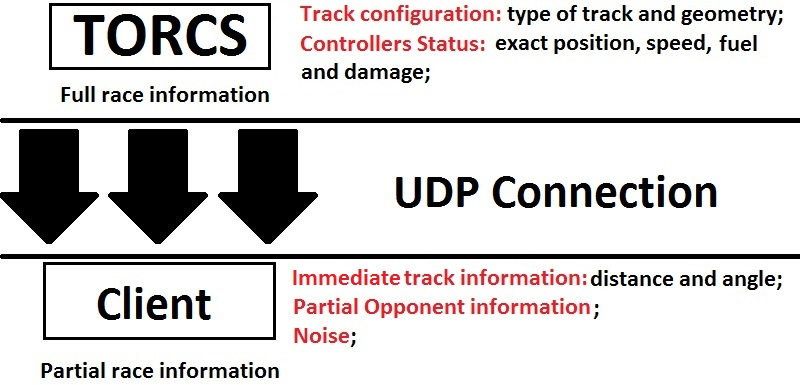
\includegraphics[width=250pt]{Figure1}
		\caption{\label{Fig:1}Available data inside TORCS and at the client.}
	\end{figure}
	
	The complete sensorial input information can be found at the Simulated Car Racing Championship Competition Software Manual~\cite{SCRC}. Noise can be introduced in the sensors, option that is present during the actual competition.

	Race tracks are categorized into \emph{Road}, \emph{Dirt} and \emph{Oval} inside TORCS. The races from the SCRC take place in track types decided by the organization of the championship, information which is not provided to the participants and that may incorporate maps that are unknown to them. The competition adopts a structure that gathers a \textit{Warm-up} stage, a \textit{Qualifier} stage and a \textit{Final} race, which are described in detail in a website of the competition~\cite{SCRC}.
	
	The reason why TORCS presents itself as a satisfactory AI benchmark, in combination with SCRC, is because even	though there are multiple possibilities on how the sensorial input received from the server can be translated into the behavior of the actuators, they can all be compared in a race, which has a robust and steady scoring and evaluational system. In other words, there are many different approaches concerning how to teach the racer encoded by the developers to drive in a racing competition only with the information given by the sensors, and the metric to that issue is the performance on the race itself.

\subsection{Related Works and State of the Art} \label{subsec:Related}
	
	It is very common among some of the SCRC awarded controllers the incorporation of machine learning in their driving methods, along with other evolving techniques using artificial intelligence. As the nature of the problematic presented comprises evolution by experience, learning procedures tend to enhance performance and competitiveness. Essentially, there are two ways of evolving controllers: Online Learning and Offline Learning, the first meaning that improvements are achieved during the actual race execution time and the latter that it is done after it, on the account of the developers themselves and with their own resources by analyzing the data gathered.
	
	The current champion of the SCR Championship is the controller \emph{Mr. Racer}~\cite{MrRacer}, and it has proven to be the State of the Art by winning the last three competitions that happened from 2011 to 2013. The authors of this implementation employ several heuristics and black-box optimization methods in order to reproduce the mechanisms to which human racing drivers resort, doing so by means of a modular structure. \emph{Mr. Racer} uses a Covariance Matrix Adaptation Evolution Strategy (CMA-ES), to evolve parameters offline.
	
	According to the founders of the competition~\cite{SCRC} and the authors of \emph{Mr. Racer} themselves, \emph{AUTOPIA}~\cite{AUTOPIA} is another competitive controller, with the potential to even be the best one available. \emph{AUTOPIA} implements a modular Fuzzy Architecture, whose division contains gear, steering and speed control; and it is optimized by means of a genetic algorithm for Offline Learning, and by means of landmarking the lane exit points for further speed reduction for Online Learning.
	
	These and other controller exemplifications~\cite{SCRC} served as criteria for the analysis and development of the approach presented in this paper. Aspects incorporated and adapted from them feature modularity, offline learning through genetic algorithms, online earning through landmarking and choosing sets of parameters for different categories of tracks, etc. Aspiring to design a controller capable of incorporating these features, the design of a model was proposed and is presented in the succeeding section.
	